\documentclass[12pt]{article}

\setlength\parindent{0pt}
\newcommand{\myt}[1]{\textbf{\underline{#1}}}

\usepackage{mathtools}
\usepackage{amssymb}

\title{\vspace{-15ex}Math 239 Lecture 27\vspace{-1ex}}
\date{July 13, 2015}
\author{Graham Cooper}

\begin{document}
	\maketitle
	
	\section*{Platonic Solids}
	
	Platonic graph, planar, vertices have the same degree, faces have the same degree\\
	$d_v$ = vertex degree\\
	$d_f$ = face degree\\
	
	\section*{Non-Planar Graphs}
	To prove that a graph is planar, we give a planar embedding\\
	
	\myt{Theorem:} When $n \geq 3$ a connected planar graph with n vertices has at most 3n-6 edges\\
	
	\myt{Proof:} Let G be a planar graph with a planar embedding with $n \geq 3$ in edges, S faces. We claim that every face has degree at least 3. If G is not a tree, then G has at least one cycle. So every face contains a cycle, which has at least 3 edges. So each face has degree $\geq$ 3. If G is a tree, then it has only once face. Its degree must be twice the number of edges, 2(n-1) = 2n-2 (by handshaking lemma for faces). Since $n \geq 3, 2n-2 \geq 3$. This proves the claim.\\
	
	Using Handshaking Lemma for faces, \\
	2m = $\sum_{f \in F} deg(f) \geq \sum_{f \in F}3 = 3S$\\
	$m \geq \frac{3}{2}S$\\
	By Euler's formula: (n-m+s = 2)\\
	$= \frac{3}{2}(2-n+m)$\\
	$= 3 - \frac{3}{2}n + \frac{3}{2}m$\\
	$\implies \frac{3}{2}n - 3 \geq \frac{1}{2}m$\\
	$\implies 3n - 6 \geq m$\\
	
	\myt{Corollary:} $K_5$ is not planar\\
	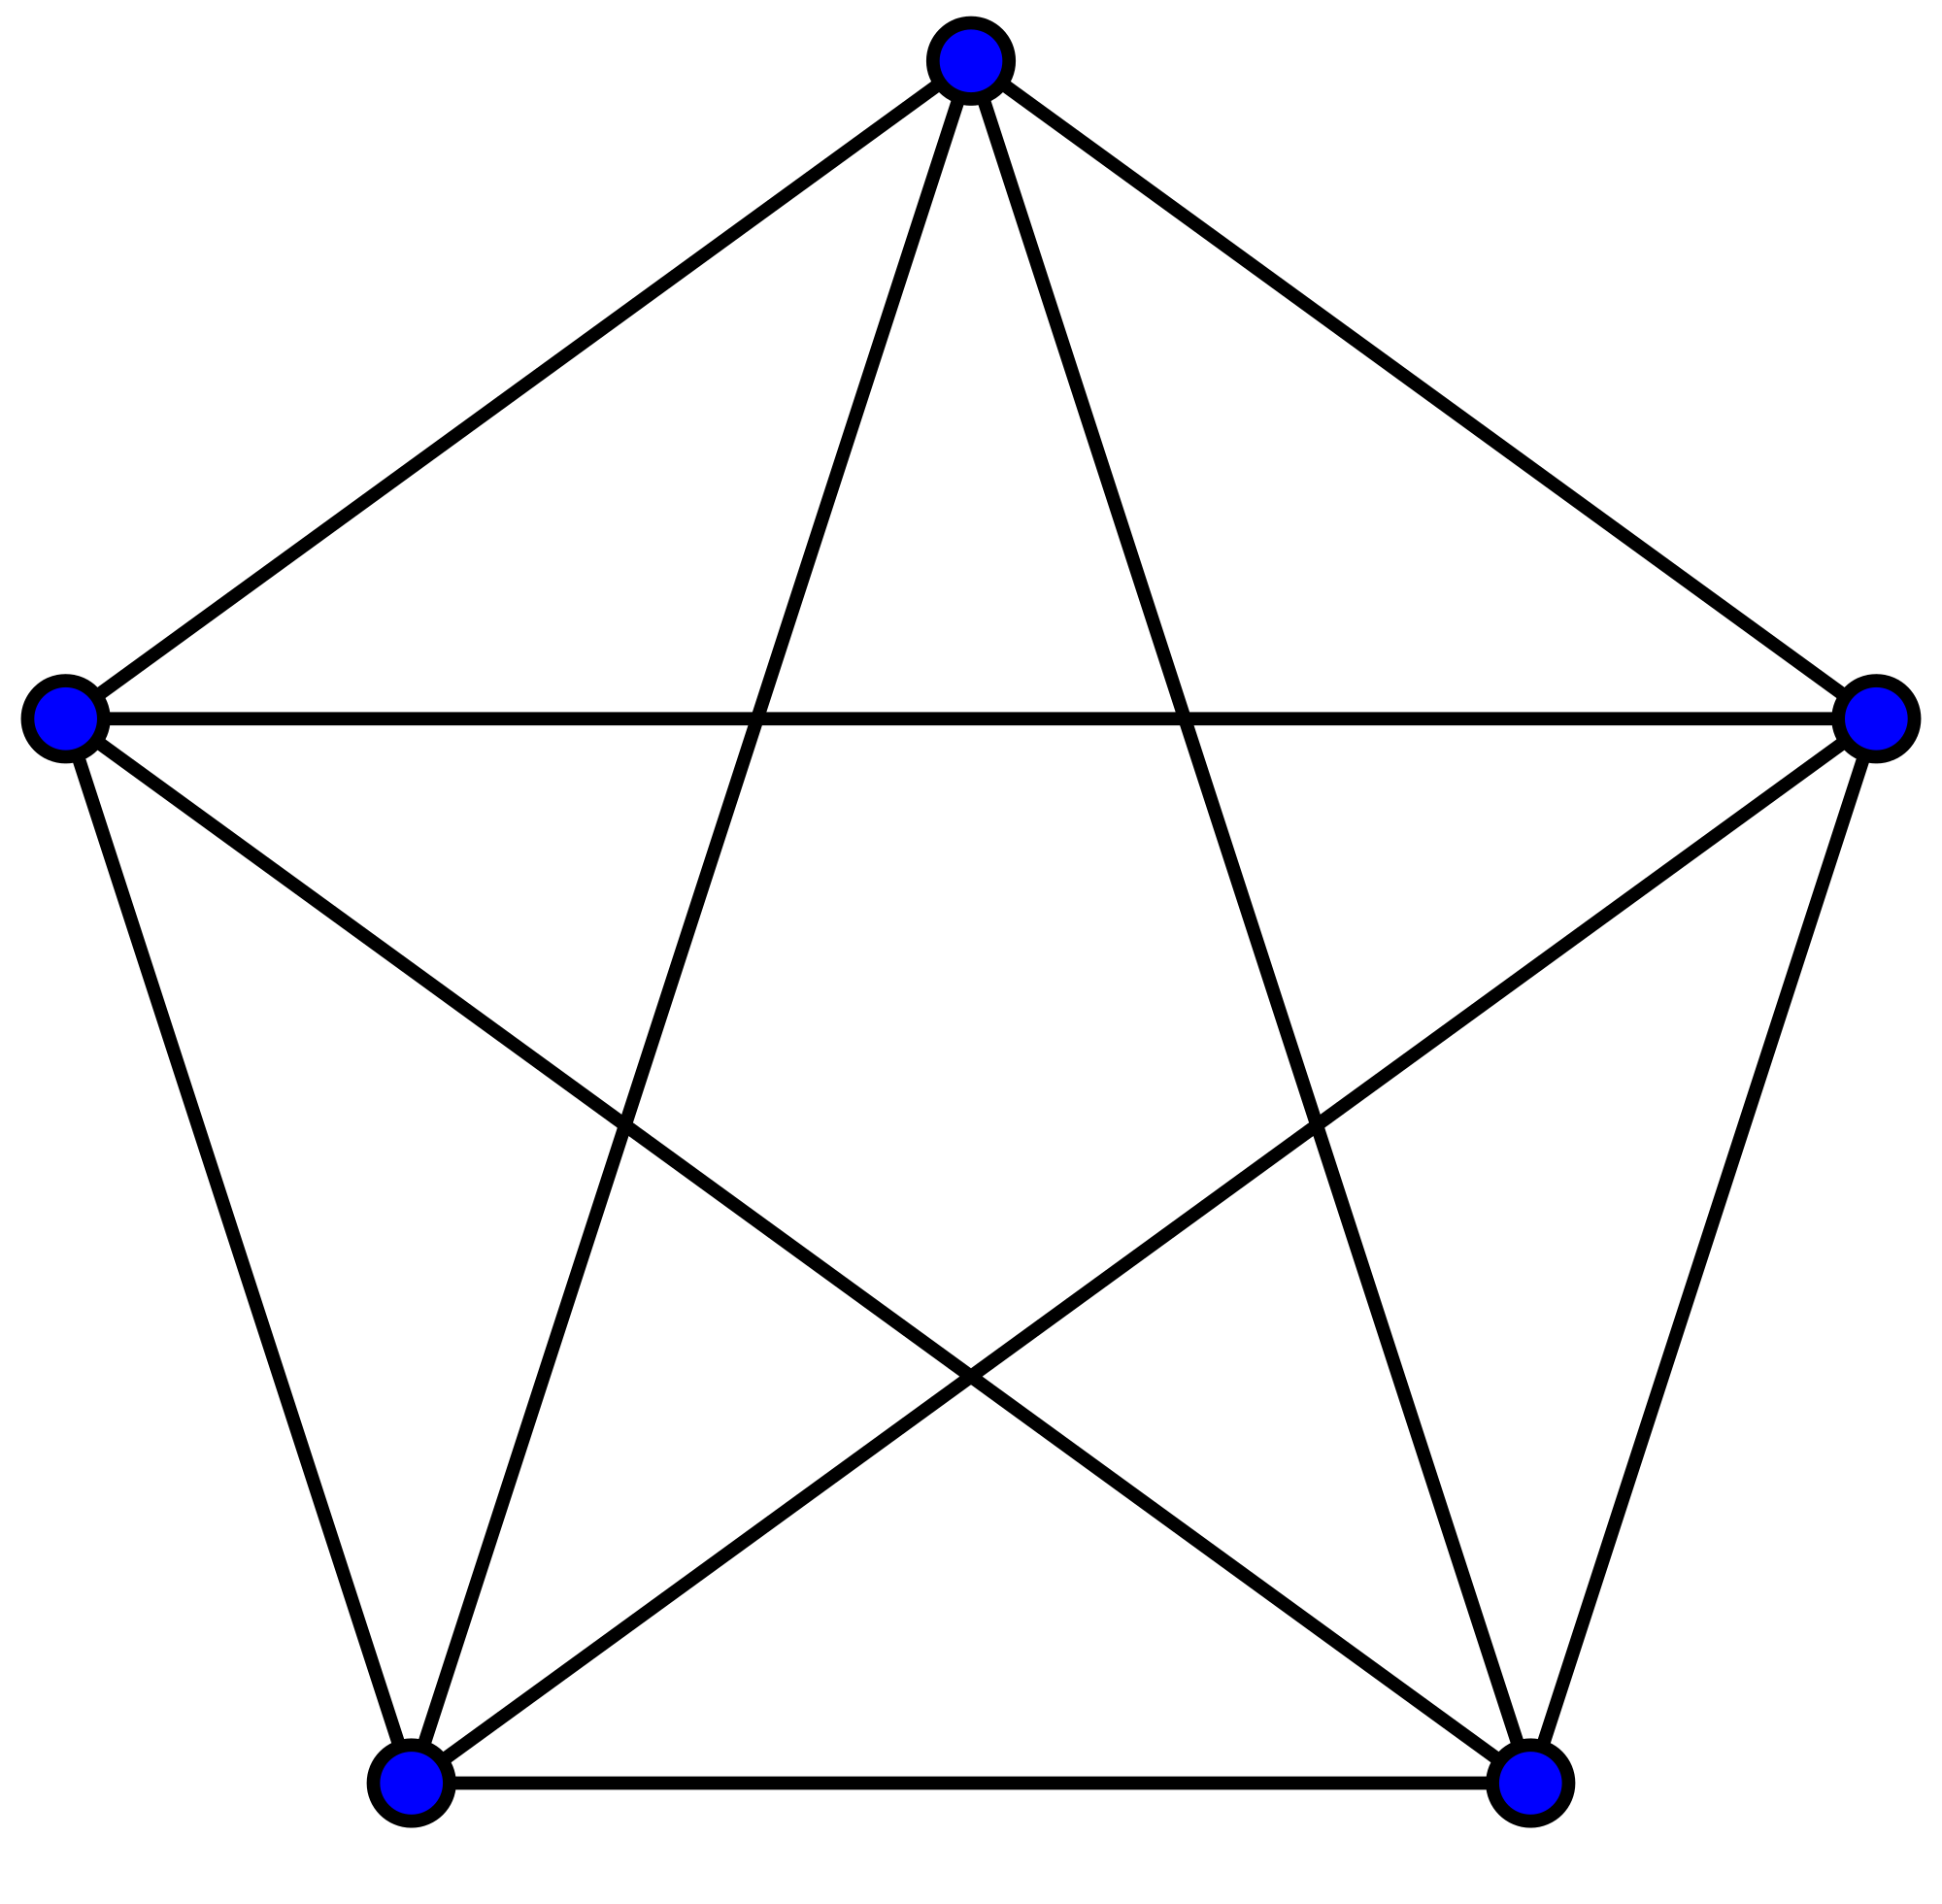
\includegraphics[scale=0.5]{k5.png}\\
	
	\myt{Proof:} $K_5$ has 5 vertices and 10 edges. Any planar graph wiht 5 vertices has at most $3 \cdot 5$- 6 = 9 edges. So $K_5$ is not planar\\
	
	The converse of the theorem is false\\
	
	\myt{Theorem:} when n $\geq$ 3, a connected bipartite planar graph with n vertice has at most 2n-4 edges\\
	
	\myt{Proof:} (Similar to the proof of hte previous thoerem)\\
	IF G has a cycle, then every face is bounded by a cycle of length $\geq$ 4 (since no triangle exists in a bipartite graph)\\
	If G is a tree, its only face has deg 2n - 2 $\geq$ 4. Since n $\geq$ 3. \\
	Using Hand shaking lemma for faces,\\
	 2m $\geq$ 4s = 4(2-n+m)\\
	 = 8 - 4n+4m\\
	 $\implies$ 4n-8 $\geq$ 2m\\
	 $\implies$ 2n-4 $\geq$ m\\
	 
	 \myt{Corollary:} $k_{3,3}$ has 6 vertices and 9 edges. Any planar bipartite graph with 6 vertices has at most $2 \cdot 6 - 4 = 8$ edes. So $k_{3,3}$ is not planar\\
	
	
	
	
\end{document}
